% \chapter{Spin states of the Dirac cone}
\section{Spin states of the Dirac cone}
Similar to the discussion in \cref{sec:spin-orbit} on the spin structure of a system with Rashba coupling, we here consider the spin structure of the Weyl cone.
We begin by finding the eigenstates of the Weyl Hamlitonian \( H = v_F \vec{\sigma} \vec{p} \).
Assume plane wave states, and some arbitrary linear combination of spin up and spin down,
\[
  \psi _{\pm} = e^{i \vec{k} \vec{r}} \alpha
  \begin{pmatrix}
    1\\
    b
  \end{pmatrix},
\]
where \(\alpha \) is some normalization.
Solving the time independent Schrodinger equation
\[
H \psi = E \psi,
\]
we find
\begin{equation}
  \label{eq:132}
  b = -\frac{k_{z} \pm k}{k_{x} - i k_{y}}.
\end{equation}
Requiring normalized states \(\braket{\psi | \psi } = 1\) gives the normalization
\[
|\alpha |^2 = \frac{1}{1 + |b|^2}.
\]

Having found the states, we find the spin expectation value
\begin{equation}
  \label{eq:133}
  \vec{S} = \braket{\psi | \hat{S} | \psi },
\end{equation}
where \(\vec{S}\) is the spin expectation value and \(\hat{S} = \frac{\vec{\sigma}}{2} \) is the spin operator, where \(\hbar \) was set to 1.
Simply evaluating \cref{eq:133}, yields
\begin{equation}
  \label{eq:134}
  \vec{S} = \pm \frac{\vec{k}}{2 k}.
\end{equation}

The spin structure is that of a hedgehog.
This gives a nice intuitive explanation of the symmetries of a Dirac cone.
Recall that under an inversion transformation, momentum is flipped while spin is invariant.
Under time-reversal both momentum and spin change direction.
When all symmetries are present, the Dirac cone consists of two superimposed Weyl cones.
Breaking inversion symmetry separates the cones in momentum while breaking time-reversal symmetry separates the cones in energy\footnote{Giving a nodal loop.}.
The three cases are shown schematically in \cref{fig:spinStructure}.
By inspection, one sees that when the cones are separated in momentum, the spin at the opposite momentum has the same direction, and so time-reversal symmetry is broken.
Similarly, when the cones are separated in energy, the spin at the opposite momentum has the opposite direction, and so inversion symmetry is broken.


\begin{figure}[p]
  \centering
  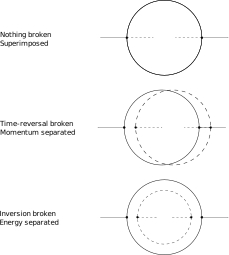
\includegraphics[width=0.75\textwidth]{figures/spinStructureWeyl}
  \caption{\label{fig:spinStructure}%
    Schematic overview of symmetry properties of a Dirac cone.
    Drawn is the energy contour of a Dirac cone for some non-zero energy;
    in other words, the intersection of a Dirac cone with a plane at some energy \( E \neq 0 \).
    The arrows indicate the spin direction.
    From top to bottom, there is a Dirac cone with two superimposed Weyl cones, momentum separated Weyl cones, and energy separated Weyl cones.
    The solid and dashed lines corresponds to the two chiralities.
  }
\end{figure}
